\documentclass[times, twoside, watermark]{style}
\usepackage{blindtext}
\usepackage{empheq}
\usepackage{tikz}
\usepackage{pgfplots} 
\usepackage{subcaption}

\leadauthor{Quentin Brateau} 

\begin{document}

\title{Magnetic mapping using a trailed magnetometer}
\shorttitle{MagMap}

% Use letters for affiliations, numbers to show equal authorship (if applicable) and to indicate the corresponding author
\author[1,\Letter]{Quentin Brateau}

\affil[1]{ENSTA Bretagne, Brest}

\maketitle

%TC:break Abstract
%the command above serves to have a word count for the abstract
\begin{abstract}
    The realization of a magnetic map of a terrain is a powerful tool especially used in mine warfare. This cartography can be done with a magnetometer, but the task is quite difficult. This is why it is useful to use robots to make this cartography. The problem induced by this solution is the addition of magnetic disturbances related to the structure of the robot and its actuators. It is then possible to drag the magnetometer on a sled behind the robot. 
\end {abstract}
%TC:break main
%the command above serves to have a word count for the abstract

\begin{keywords}
Magnetic | Mapping | Control | Interval Analysis
\end{keywords}

\begin{corrauthor}
%\texttt{r.henriques{@}ucl.ac.uk}
quentin.brateau\at ensta-gretagne.org
\end{corrauthor}

\section*{Modelisation of the system}
    The system is composed of a vehicle that will drag a sledge that transports a magnetometer. The towing vehicle is a tank type vehicle, and the sled is attached to it with a rope. Assuming that the rope is constantly under tension, we are able to find the equations describing the dynamics of the system. By noting $x$ the state of the system and $u$ its inputs, the dynamics of the system is described by :

    \begin{empheq}[left={\dot{x} = f(x, u) =}\empheqlbrace]{align}
        \dot{x_1} &=\ \dfrac{u_1 + u_2}{2}.cos(x_3) \label{eq:x}\\
        \dot{x_2} &=\ \dfrac{u_1 + u_2}{2}.sin(x_3) \label{eq:y}\\
        \dot{x_3} &=\ u_2 - u_1 \label{eq:theta}\\
        \dot{x_4} &=\ - \dfrac{u_1 + u_2}{2}.sin(x_4) - \dot{x_3} \label{eq:phi}
    \end{empheq}


\section*{Simulator}
    A python simulation was realized using VIBES in order to test the behavior of the system. A class \textit{Tank} has been created to instantiate a vehicle with its sled. Then the script integrates the evolution equation using Euler's method in order to obtain the state of the system $x$ according to the $u$ inputs. We could see that the behavior of the system seems correct and the model is faithful to reality. Moreover, the GNSS sensor and an accelerometer are simulated in order to enclose the real position in a box.

    \begin{figure}[!htb]
        \centering
        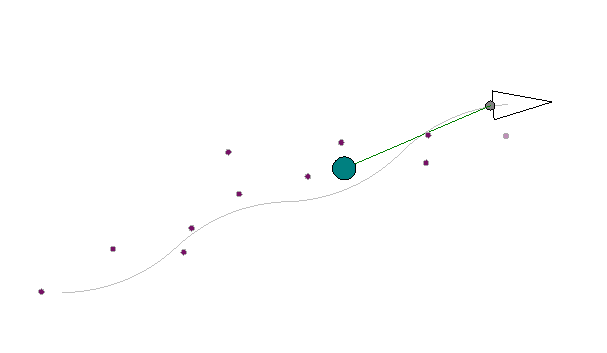
\includegraphics[width=0.4\textwidth]{imgs/simulator.png}
        \caption{\label{fig:simulation} Simulation of the system}
    \end{figure}

\section*{Reliable set of sled's angle}
    Considering that the rope remains continuously under tension while the robot is moving, then the evolution of the angle $x_4$ of the sled relative to the towing vehicle is described by the \textit{Differential Equation}~\ref{eq:phi}.

    We are able to find the trajectory of the sled by computing the interval containing the angle $x_4$, considering that initially $x_4$ belongs to $[-\pi/2; \pi/2]$. Then by applying the \textit{Differential Equation}~\ref{eq:phi} on this interval, we end up obtaining a fine interval framing the real angle $x_4$, independently of the initial angle as we can see on the \textsc{Figure}~\ref{fig:integration}.

    \begin{figure}[!htb]
        \centering
        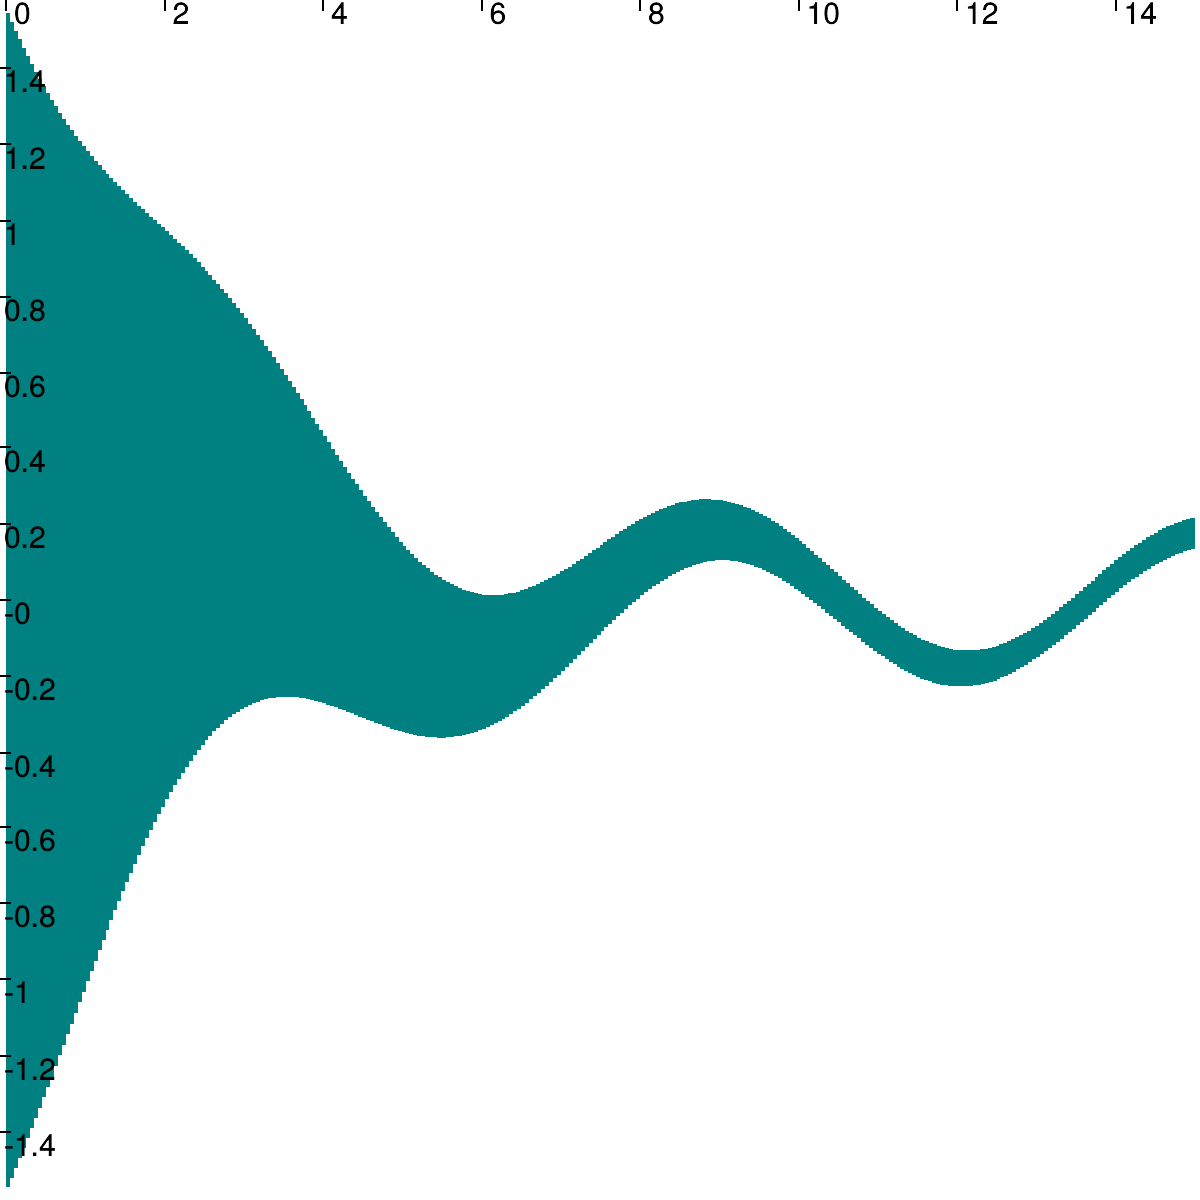
\includegraphics[width=0.35\textwidth]{imgs/integration_example.png}
        \caption{\label{fig:integration} Integration example using intervals}
    \end{figure}

\section*{Sled localization}
    Considering that the rope remains continuously under tension while the robot is moving, then the evolution of the angle $x_4$ of the sled relative to the towing vehicle is described by the \textit{Differential Equation}~\ref{eq:phi}.

    Then we are able to find the trajectory of the sled by calculating the interval containing the angle $x_4$. The idea is to consider that initially $x_4$ belongs to $[-\pi/2; \pi/2]$. Then by applying \textit{Equation}~\ref{eq:phi} on this interval, we end up obtaining a fine interval framing the real angle $x_4$, independently of the initial angle as we can see on the \textsc{Figure}~\ref{fig:integration}.

    \begin{figure}[!htb]
        \centering
        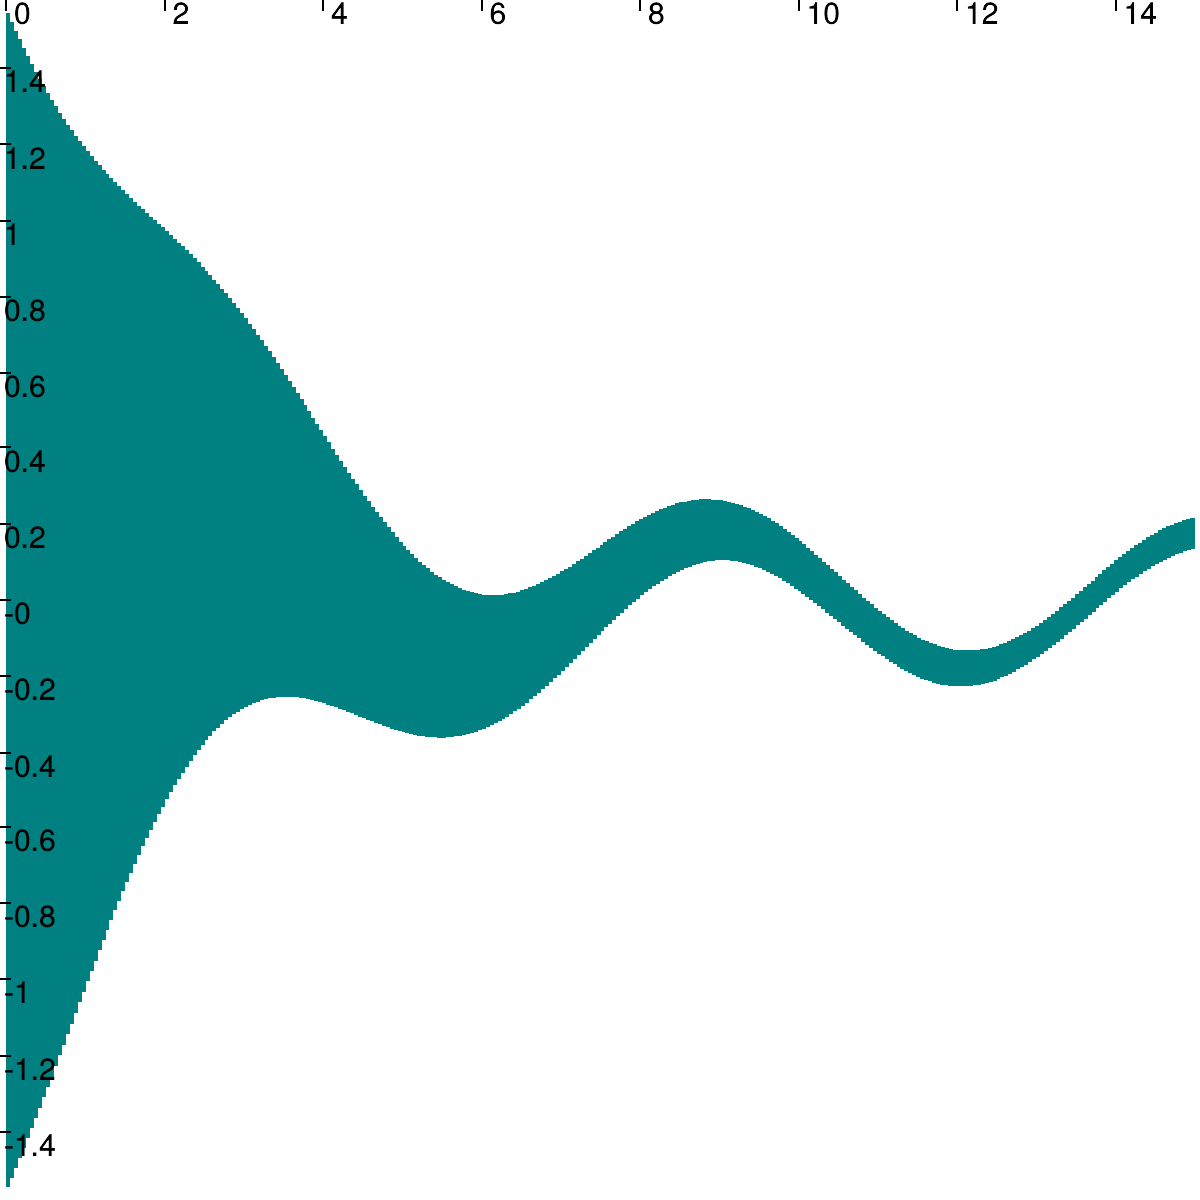
\includegraphics[width=0.35\textwidth]{imgs/integration_example.png}
        \caption{\label{fig:integration} Integration example using intervals}
    \end{figure}

    By having an interval framing the angle $x_4$, we are able to obtain a box containing the sled, knowing the length of the rope.
    This box has the shape of a pie sector. \textit{Equation}~\ref{eq:magnetometer} presents the position of the magnetometer as a function of the state of the system $x_1$, $x_2$ and $x_4$. Here all these variables are intervals. By applying a polar contractor to these intervals, we are able to obtain the intervals containing $x_m$ and $y_m$.

    \begin{equation}\label{eq:magnetometer}
        \left\lbrace
            \begin{aligned}
                x_m &= x_1 - L.cos(x_4) \\
                y_m &= x_2 - L.sin(x_4)
            \end{aligned}
        \right.
    \end{equation}

\section*{Magnetometer range of measurement}
    By knowing a box containing the magnetometer and its measuring range, we are able to find all the points seen for sure and all the points that could be seen by the magnetometer. This allows us to recover the coverage of the area by the magnetometer.

    \begin{figure}[!htb]
        \centering
        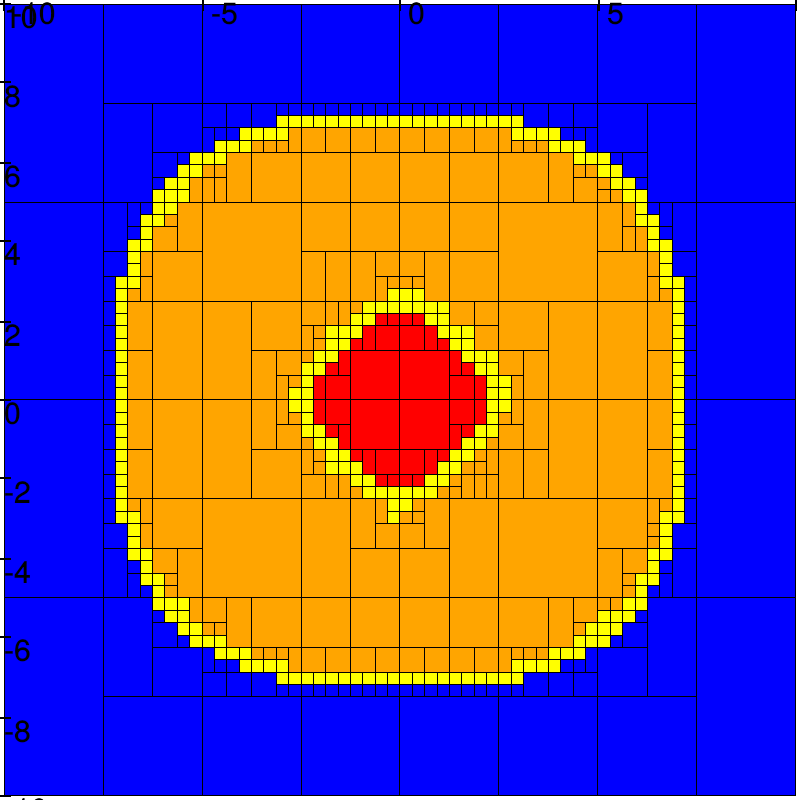
\includegraphics[width=0.4\textwidth]{imgs/thickset.png}
        \caption{\label{fig:thickset} Measurement range of the magnetometer using Thicksets}
    \end{figure}

    The \textsc{Figure}~\ref{fig:thickset} shows us these two sets. The blue set is the unseen area, the orange set is the area maybe seen and the red set is the area seen for sure by the magnetometer. The yellow set forms the uncertain boundary between the other sets, which can be adjusted. Thus we have a way to know precisely the coverage of the mapping during the mission.

\section*{Magnetometer Mapping}
    With a moving box enclosing the magnetometer at any time, this method allows us to recover the coverage of the area by the magnetometer. Thus we have a way to know precisely the coverage of the mapping during the mission, which depends on the uncertainty on the position of the magnetometer and on the maximum distance of each point of the field to be measured. An example of the covered area of a magnetometer on a field is presented by the \textsc{Figure}~\ref{fig:thickset_trajectory}.

    \begin{figure}[!htb]
        \centering
        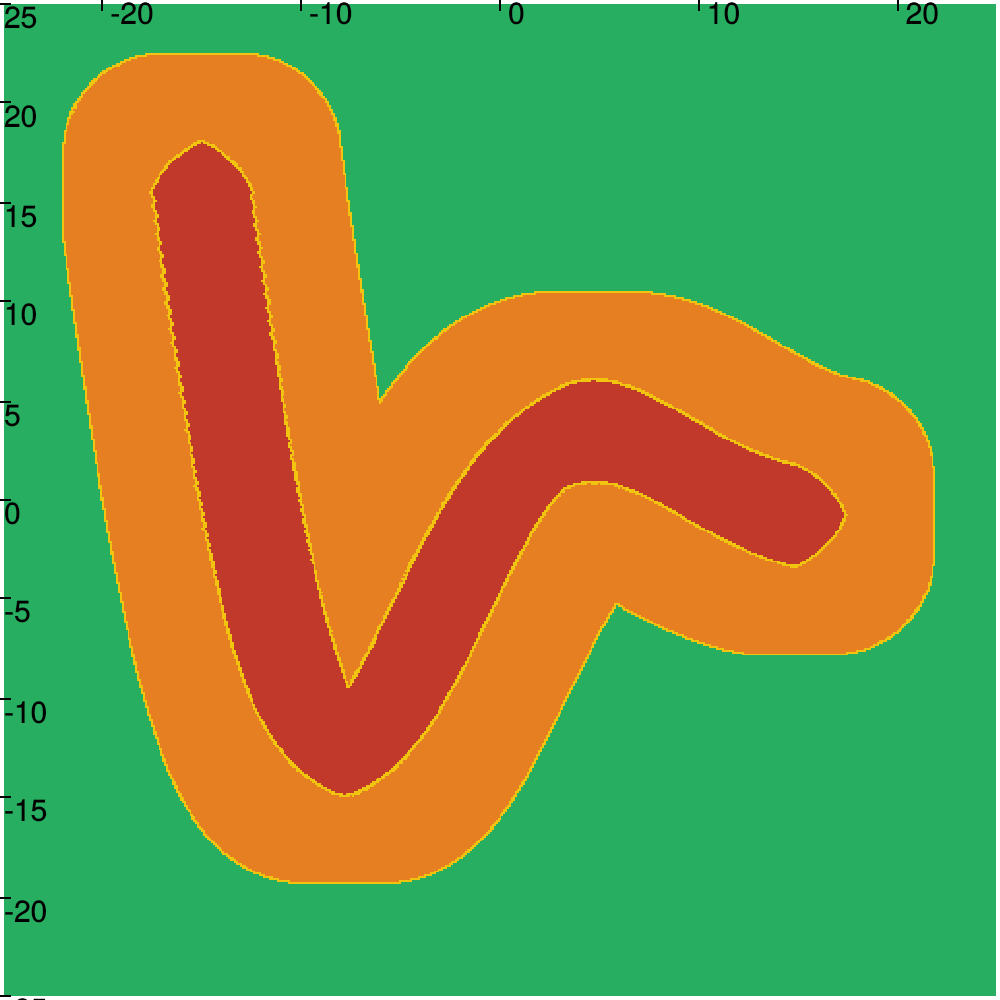
\includegraphics[width=0.4\textwidth]{imgs/thickset_fine_cmap.png}
        \caption{\label{fig:thickset_trajectory} Coverage of the map by the magnetometer using Thicksets}
    \end{figure}
    
    

\section*{Application example}
    Having inputs $U$ and some dated inertial and GNSS measurements $G$, we are able to get a tube enclosing the trailing robot, available on \textsc{Figure}~\ref{fig:trailing}, and a tube enclosing the magnetometer, available on \textsc{Figure}~\ref{fig:magneto}. The estimated angle of the sled according to the trailing vehicle is also showed on the \textsc{Figure}~\ref{fig:phi}.

    \begin{figure}[!htb]
        \begin{subfigure}{0.5\textwidth}
            \centering
            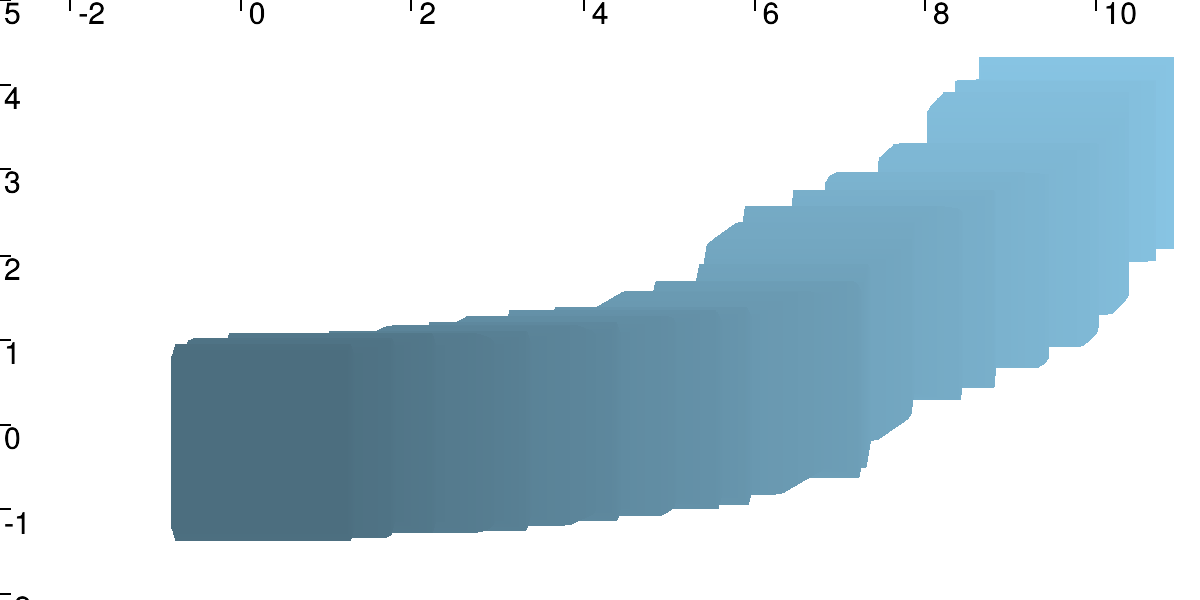
\includegraphics[width=0.8\textwidth]{imgs/example_saturne.png}
            \caption{Trailing robot enclosing tube}
            \label{fig:trailing}
            \hfill
        \end{subfigure}
        \newline
        \begin{subfigure}{0.5\textwidth}
            \centering
            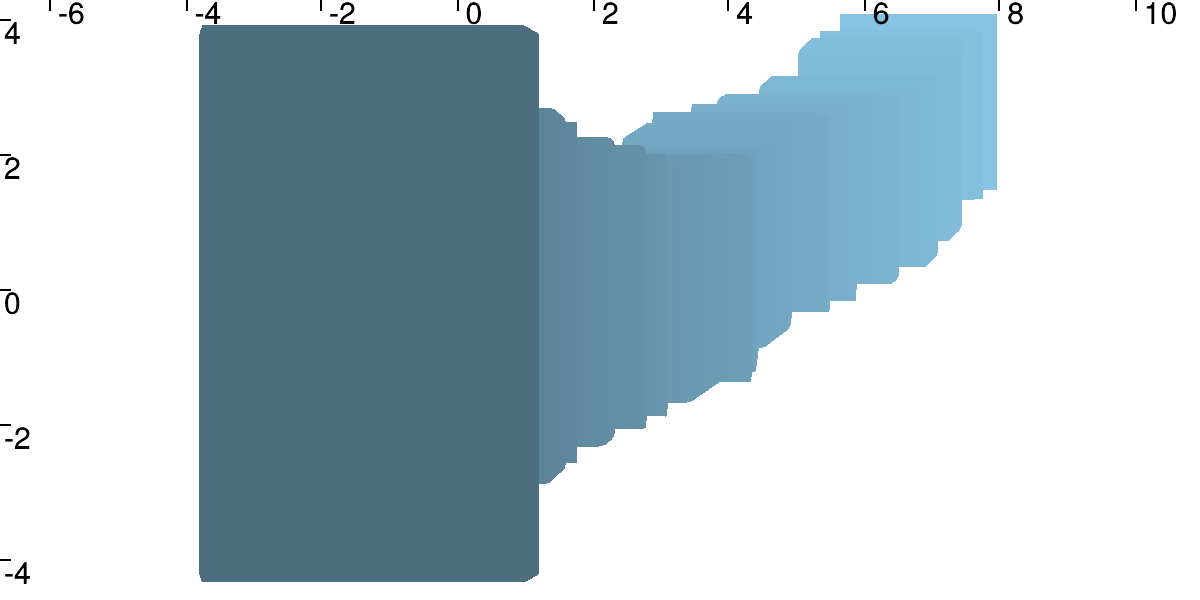
\includegraphics[width=0.8\textwidth]{imgs/example_magnetometer.png}
            \caption{Magnetometer enclosing tube}
            \label{fig:magneto}
            \hfill
        \end{subfigure}
        \newline
        \begin{subfigure}{0.5\textwidth}
            \centering
            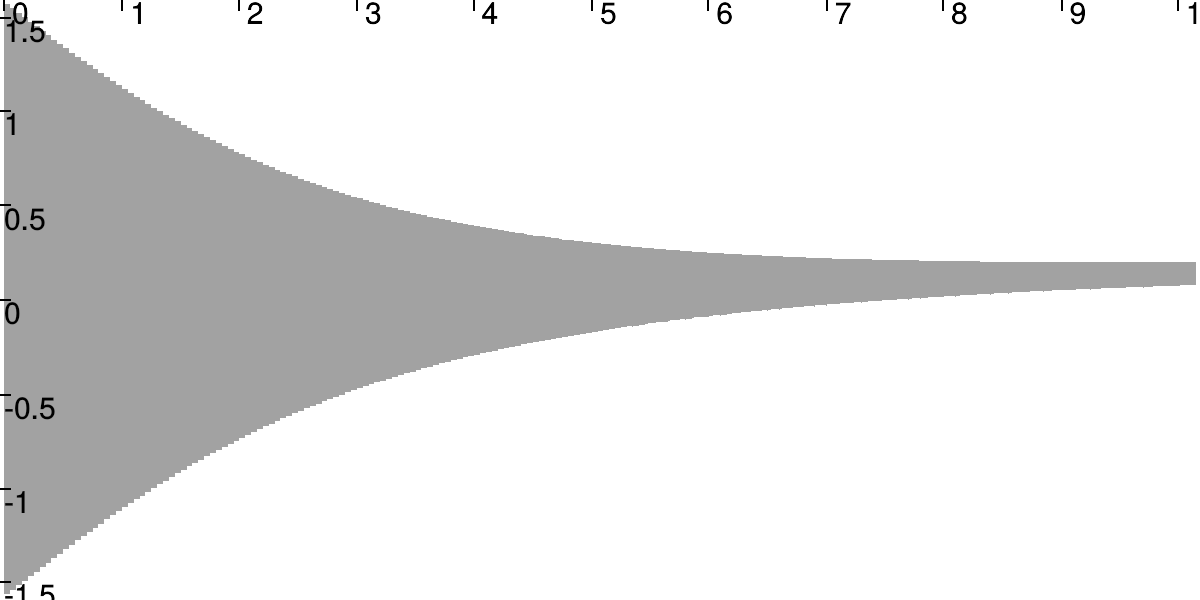
\includegraphics[width=0.8\textwidth]{imgs/example_phi.png}
            \caption{Sled angle estimation}
            \label{fig:phi}
            \hfill
        \end{subfigure}
        \caption{\label{fig:example_tube} Example of enclosing tube}
    \end{figure}
    \hfill

    We could see that the $\phi$ angle is quickly bounded regardless of knowing the initial condition. It let us have a more precise box enclosing the magnetometer. Finally, we are able to have a mapping of the coverage of the magnetometer visible on the \textsc{Figure}~\ref{fig:example_coverage}. Initially the uncertainty on the position of the magnetometer being large, the set of points that can be seen is large and the set of points seen for sure is very small. Then as the robot moves forward, the position of the magnetometer is better known and the set of points seen for sure is increasing.

    \begin{figure}[!htb]
        \centering
        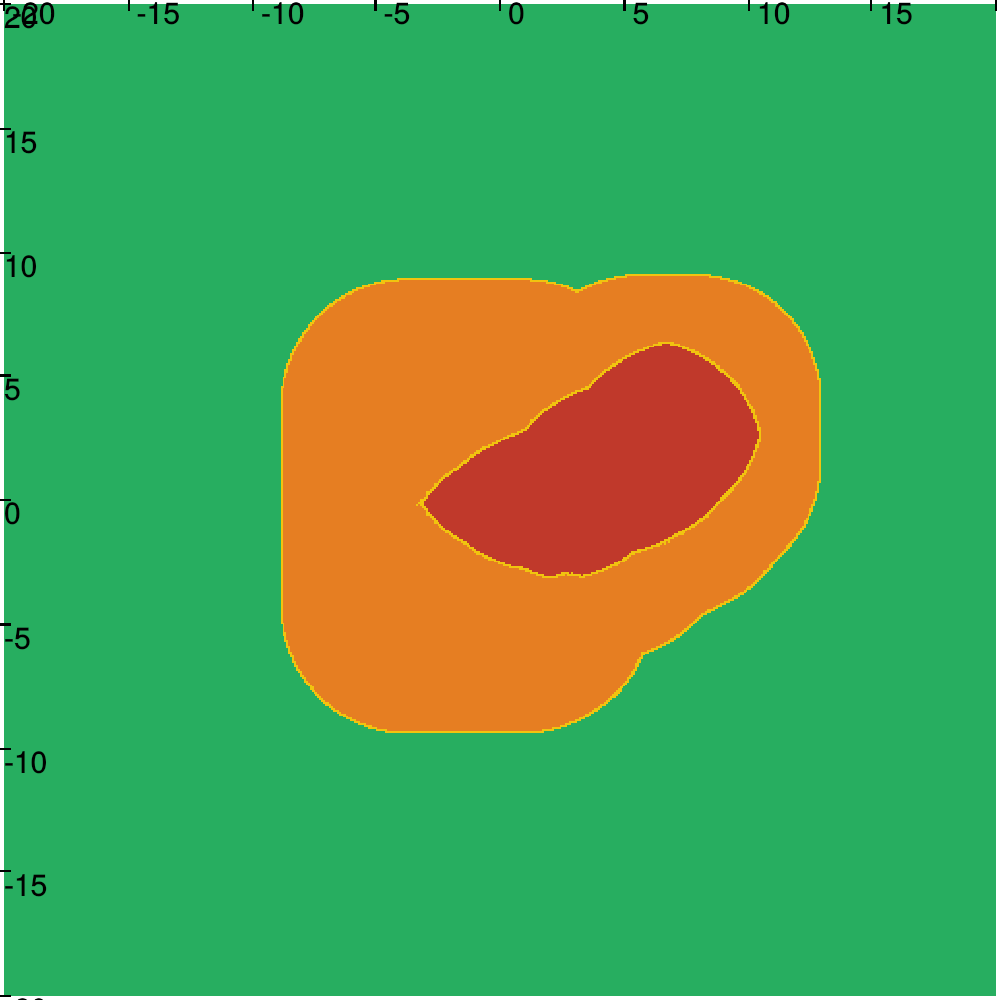
\includegraphics[width=0.4\textwidth]{imgs/example_coverage.png}
        \caption{Mapping coverage}
        \label{fig:example_coverage}
    \end{figure}



% \begin{acknowledgements}
% \blindtext
% \end{acknowledgements}

% \section*{Bibliography}
% \bibliography{zHenriquesLab-Mendeley}

% %% You can use these special %TC: tags to ignore certain parts of the text.
% %TC:ignore
% %the command above ignores this section for word count
% \onecolumn
% \newpage

% \section*{Word Counts}
% This section is \textit{not} included in the word count. 
% \subsection*{Notes on Nature Methods Brief Communication}
% \begin{itemize}
% \item Abstract: 3 sentences, 70 words.
% \item Main text: 3 pages, 2 figures, 1000-1500 words, more figures possible if under 3 pages
% \end{itemize}

% \subsection*{Statistics on word count}
% \detailtexcount
% \newpage

%%%%%%%%%%%%%%%%%%%%%%%%%%%%%
% Supplementary Information %
%%%%%%%%%%%%%%%%%%%%%%%%%%%%%
% \captionsetup*{format=largeformat}
% \section{Something about something} \label{note:Note1} 
% \Blindtext

%TC:endignore
%the command above ignores this section for word count

\end{document}